\maketitle
\tableofcontents
\newpage

\section{Zielsetzung}
Ziel des Versuches ist die Bestimmung der Temperaturabhängigkeit der dynamischen
Viskosität von destilliertem Wasser mithilfe des Kugelfall-Viskosimeters nach Höppler.
\section{Theorie}
Bei Bewegung durch Flüssigkeiten erfahren Körper eine Reibungskraft, die von der
Berührungsfläche A und der Geschwindigkeit $v$ abhängt. Eine weitere wichtige Rolle
spielt die $\textbf{dynamische Viskosität}$, eine Eigenschaft der Flüssigkeit, die
temperaturabhängig ist. Mithilfe des $\textbf{Kugelfall-Viskosimeters nach Höppler}$
lässt sich Diese bestimmen. Wenn der Radius der Kugel sich nur marginal von dem
der Röhre unterscheidet, sodass sich keine Turbulenzen bilden, dann gilt für die
Stokessche Reibung
\begin{equation}
  F_R = 6 \, \pi \, \eta \, v \, r \ .
\end{equation}
$r$ ist hierbei der Radius der Kugel und $\eta$ die dynamische Viskosität.
Wenn die Kugel im Rohr hinabfällt, wirken neben der Reibungskraft auch die
Schwerkraft und die Auftriebskraft. Da die Reibungskraft immer entgegen
der Bewegungsrichtung wirkt und die Auftriebs- und Schwerkraft auch entgegengesetzt
wirken, arbeiten also Auftriebs und Reibungskraft egegen die Schwerkraft.
Es stellt sich nach einiger Zeit ein Kräftegleichgewicht ein, da die Reibungskraft
von der Geschwindigkeit $v$ abhängt. Somit fällt die Kugel mit konstanter Geschwindigkeit.
Bei einem senkrechten Fall würde die Kugel mit den Wänden der Röhre kollidieren und so
Wirbel verursachen. Deswegen wird das Rohr um einige Grade geneigt, sodass die Kugel
auf der Oberfläche gleiten kann.

Die Viskosität bestimmt sich nach folgender Formel
\begin{equation}
  \eta = K (\rho_K - \rho_{Fl}) \cdot t \ .
  \label{eqn:4}
\end{equation}
Hierbei ist $t$ die Fallzeit der Kugel, $\rho_K$ und $\rho_{Fl}$ die Dichten
der Kugel bzw. der Flüssigkeit. Die Apparaturkonstante $K$ setzt sich unter anderem
aus Fallhöhe und der Kugelgeometrie zusammen.

Da die Viskosität vieler Flüssigkeiten auch von der Temperatur abhängig ist, gibt die
Andradesche Gleichung eine Abhängigkeit der Viskosität von der Temperatur an
\begin{equation}
  \eta(T) = A \ exp\left(\frac{B}{T}\right) \ .
  \label{eqn:5}
\end{equation}
Mithilfe der Reynoldszahl\cite[99]{geschke}
\begin{equation}
  Re = \frac{\rho \, v \, d}{\eta}
  \label{eqn:6}
\end{equation}
lässt sich eine Aussage darüber treffen, ob eine Strömung laminar, also turbulenzfrei,
ist oder ob sie Wirbel hat. Alle Werte, die unter der Reynoldszahl liegen, sind laminare
Strömungen, alle, die darüber liegen sind es nicht.

\section{Durchführung}
\subsection{Versuchsaufbau}
\label{sec:3.1}
\begin{figure}
  \centering
  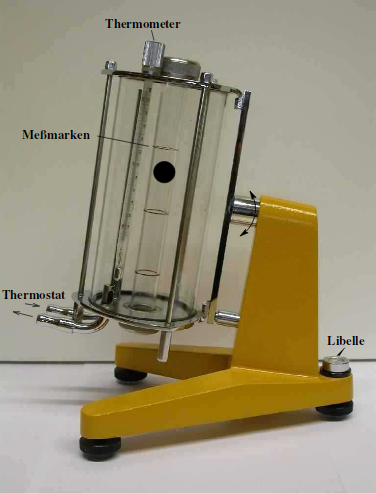
\includegraphics[scale=0.4]{visko.png}
  \caption{Ein Kugelfall-Viskosimeter nach Höppler.}
  \label{fig:1}
\end{figure}
In Abbildung \ref{fig:1} ist ein Kugelfall-Viskosimeter nach Höppler zu sehen.
Im Inneren befindet sich die erwähnte Röhre, die drei Messmarkierungen aufweist.
Die Fallstrecke zwischen der obersten und der untersten beträgt $\SI{0.1}{\meter}$.
Das Rohr lässt sich von beiden Seiten mit der Flüssigkeit und einer Kugel befüllen.
Um die Temperaturabhängigkeit zu beobachten, kann die Flüssigkeit im Rohr mit einem Wasserbad
temperieren, siehe Abbildung \ref{fig:2}. Mithilfe der Libelle lässt sich sicherstellen,
dass das Viskosimeter gerade steht.
\begin{figure}
  \centering
  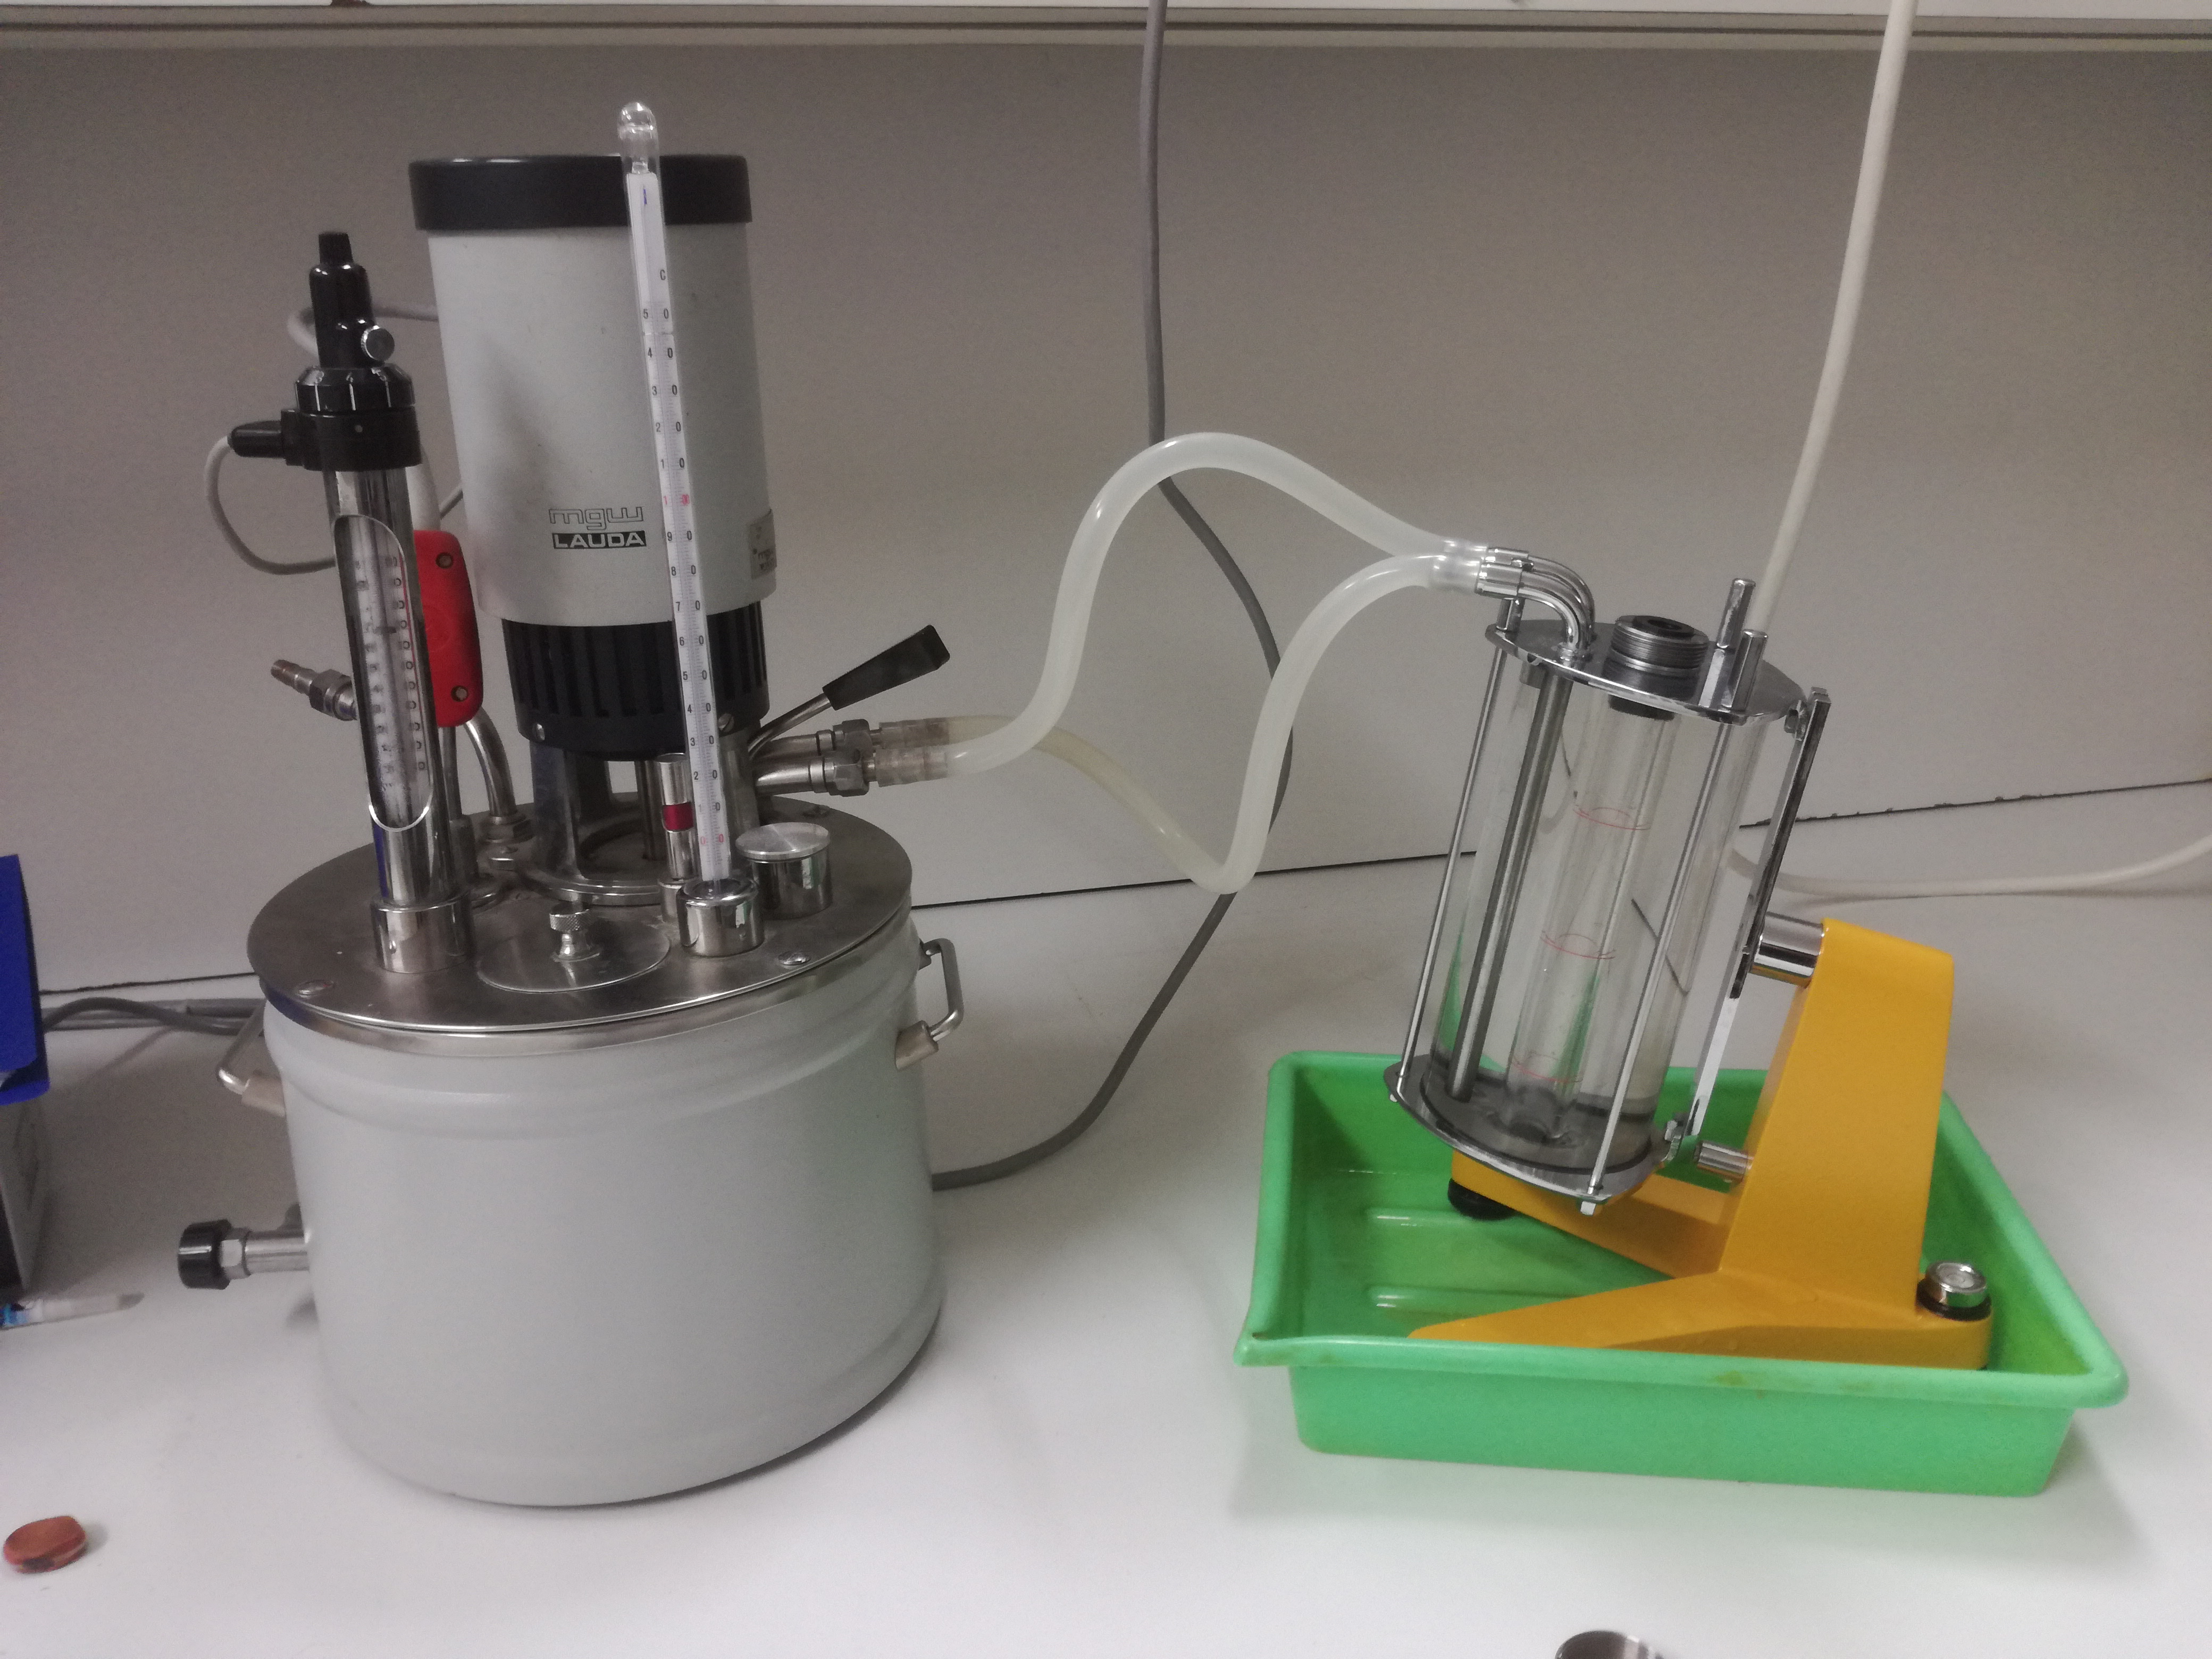
\includegraphics[scale=0.05]{aufbau.jpg}
  \caption{Versuchsaufbau im Foto.}
  \label{fig:2}
\end{figure}
\subsection{Versuchsdurchführung}
Als erstes wurde mithilfe eines  Messschiebers die Durchmesser der zwei Kugeln
fünfmal bestimmt. Ebenso oft wurden die Kugeln gewogen, um aus Volumen und Gewicht
die Dichte $\rho_{K}\footnote{siehe \eqref{eqn:4}}$ zu bestimmen. Nachdem sichergestellt
wurde, dass das Viskosimeter gerade steht, wird das Röhrchen mit destilliertem Wasser
befüllt, und dabei entstehende Luftblasen entfernt. Alsdann wird mit einer Stoppuhr
die Fallzeit der Kugel auf der in Kapitel \ref{sec:3.1} beschriebenen Messstrecke
bestimmt. Wenn die Kugel unten angekommen ist, wird das Viskosimeter um $\SI{180}{\degree}$
gedreht und erneut die Fallzeit bestimmt. Dabei ist darauf zu achten, dass die Kugel
vor dem Erreichen der ersten Messmarkierung eine konstante Geschwindigkeit erreicht hat.
Für die zwei Kugeln werden jeweils zehn Messungen durchgeführt. Anschließend wird das
Wasserbad und damit das destillierte Wasser in der Röhre auf $\SI{70}{\celsius}$
geheizt. Im Zuge dessen wird ab $\SI{25}{\celsius}$ in $\SI{5}{\celsius}$ Schritten zweimal
die Fallzeit der größeren Kugel bestimmt, bis die $\SI{70}{\celsius}$ erreicht sind.

\section{Fehlerrechnung}
Es gibt:
\begin{equation}
  \bar{T} = \frac{1}{n} \sum_{i=1}^{n} T_{i}
  \label{eqn:1}
\end{equation}
den Mittelwert und:
\begin{equation}
  \sigma_{\bar{T}} = \sqrt{\frac{1}{n(n-1)} \sum_{i=1}^{n}(\bar{T}-T_i)^2}
  \label{eqn:2}
\end{equation}
den Fehler des Mittelwertes. Falls zwei fehlerbehaftete Größen in einer Gleichung
zur Bestimmung einer anderen Größe Verwendung finden, dann berechnte sich der Gesamtfehler
nach der Gaußschen Fehlerfortpflanzung zu
\begin{equation}
    \symup \Delta f(x_1, x_2, ..., x_n) = \sqrt{\left(\frac{\symup df}{\symup dx_1} \symup \Delta
    x_1 \right)^2 +    \left(\frac{\symup df}{\symup dx_2} \symup \Delta
    x_2 \right)^2 + ... + \left(\frac{\symup df}{\symup dx_n} \symup \Delta x_n \right)^2} \ .
    \label{eqn:3}
\end{equation}

\section{Auswertung}
\subsection{Bestimmung der Apperaturkonstante für die Große Kugel}
\label{sec:Apperat}
Die gemessenen Werte für Durchmesser und Gewicht sind in Tabelle \ref{tab:1}
aufgetragen.
\begin{table}[h]
  \centering
  \caption{Durchmesser und Gewicht der Kugeln, 5 Messungen}
  \label{tab:1}
  \begin{tabular}{S S S S}
    \toprule
    \multicolumn {2}{c}{Kugel 1} & \multicolumn {2}{c}{Kugel 2}\\
    {$d$/\si{\milli\metre}} & {$m$/\si{\gram}} & {$d$/\si{\milli\metre}} & {$m$/\si{\gram}} \\
    \midrule
    14.43 & 4.47 & 14.60 & 4.96 \\
    14.42 & 4.46 & 14.59 & 4.95 \\
    14.44 & 4.46 & 14.60 & 4.94 \\
    14.41 & 4.46 & 14.59 & 4.96 \\
    14.42 & 4.45 & 14.58 & 4.97 \\
    \bottomrule
  \end{tabular}
\end{table}
Aufgrund der in \ref{tab:1} dargestellten Werte, wird Kugel 1 im weiteren als "kleine Kugel"
und Kugel 2 als "große Kugel" bezeichnet.
Aus diesen Messwerten folgen nach \eqref{eqn:1} und \eqref{eqn:2} die in Tabelle \ref{tab:2}
dargestellten Werte für Durchmesser $d$ und Masse $m$ der Kugeln, sowie die durch:
\begin{equation}
  \rho = \frac{m}{V}
\end{equation}
mit:
\begin{equation}
  V_{Kugel} = \frac{4}{3} \cdot \pi \cdot \left(\frac{d}{2}\right)^2
\end{equation}
definierte Dichte.
\begin{table}[h]
  \centering
  \caption{Mittelwerte für Durchmesser, Masse und Dichte der Kugeln}
  \label{tab:2}
  \begin{tabular}{c c c}
    \toprule
    & kleine Kugel & große Kugel \\
    \midrule
    $d$/\si{\milli\metre} & \num{14.424(5)} & \num{14.592(4)} \\
    $m$/\si{\gram} & \num{4.460(3)} & \num{4.956(5)} \\
    $\rho$/\si[per-mode=reciprocal]{\kilo\gram\per\cubic\metre} & \num{2838(4)} & \num{2742(3)} \\
    \bottomrule
  \end{tabular}
\end{table}
\begin{table}[h]
  \centering
  \caption{Fallzeiten bei Raumtemperatur}
  \label{tab:3}
  \begin{tabular}{c c}
    \toprule
    $t_{k}$/\si{\second} & $t_{g}$/\si{\second} \\
    \midrule
    13.23 & 87.38 \\
    13.24 & 87.35 \\
    13.20 & 88 \\
    13.13 & 89.55 \\
    13.16 & 86.01 \\
    13.21 & 86.56 \\
    12.87 & 87.54 \\
    13.09 & 88.29 \\
    12.89 & 86.86 \\
    12.76 & 86.91 \\
    \bottomrule
  \end{tabular}
\end{table}
Aus den in Tabelle \ref{tab:3} dargestellten Messwerten für die Fallzeit bei Raumtemperatur
folgt nach \eqref{eqn:4} bei einer Dichte von Wasser von $\rho_{H_2O} = \SI[per-mode=reciprocal]{997.77}{\kilo\gram\per\cubic\metre}$
und mit gegebener Apperaturkonstante $K_{kl} = \SI[per-mode=reciprocal]{7.64e-8}{\pascal\cubic\metre\per\kilo\gram}$
eine Viskosität von $\eta = \SI{1.839(9)e-3}{\pascal\second}$.
Durch einsetzen dieser Viskosität in der aus \eqref{eqn:4} folgenden Form:
\begin{equation}
  K = \frac{\eta}{(\rho_K - \rho_{Fl}) \cdot t}
\end{equation}
mit der Dichte der größeren Kugel folgt $K_{gr} = \SI[per-mode=reciprocal]{1.206(7)e-08}{\pascal\kilo\gram\per\cubic\metre}$.
\subsection{Bestimmung der Visositätsfunktion}
\begin{table}[h]
  \centering
  \caption{Fallzeiten bei verschiedenen Temperaturen, 2 Messungen}
  \label{tab:4}
  \begin{tabular}{c c c c c}
    \toprule
    $T$/\si{\kelvin} & $t_1$/\si{\second} & $t_1$/\si{\second} & $\bar{t}$/\si{\second} & $\eta(T)$/\SI{e-3}{\pascal\second} \\
    \midrule
    298.15 & 74.80 & 75.76 & 75.28 & 1.58 \\
    303.15 & 68.86 & 68.75 & 68.81 & 1.45 \\
    308.15 & 63.00 & 63.01 & 63.00 & 1.33 \\
    313.15 & 56.76 & 56.90 & 56.83 & 1.20 \\
    318.15 & 52.35 & 51.83 & 52.09 & 1.10 \\
    323.15 & 47.23 & 47.93 & 47.58 & 1.00 \\
    328.15 & 44.12 & 44.56 & 44.34 & 0.93 \\
    333.15 & 40.64 & 41.27 & 40.95 & 0.86 \\
    338.15 & 38.49 & 38.29 & 38.39 & 0.81 \\
    343.15 & 36.24 & 35.75 & 36.00 & 0.76 \\
    \bottomrule
  \end{tabular}
\end{table}
Die gemessenen Werte sowie der aus den jeweils zwei Messungen folgende Mittelwert
und die mit den in Kapitel \ref{sec:Apperat} bestimmten Konstanten aus \eqref{eqn:4} folgenden
Viskositäten finden sich in Tabelle \ref{tab:4}. Die Fehler der Viskositäten sind im Bereich von $10^6$
und damit zu Vernachlässigen. Werden die Werte der Viskositäten nun logarithmiert und gegen
$1/T$ aufgetragen, lassen sich die Koeefizienten aus \eqref{eqn:5} durch folgende Form
ermitteln:
\begin{equation}
  ln(\eta(T)) = ln(A) + B * \frac{1}{T}
\end{equation}
Dazu wird ein linear Fit auf den Daten angewendet. Dies ist in Grafik \ref{plot:1} dargestellt.
\begin{figure}[h]
  \centering
     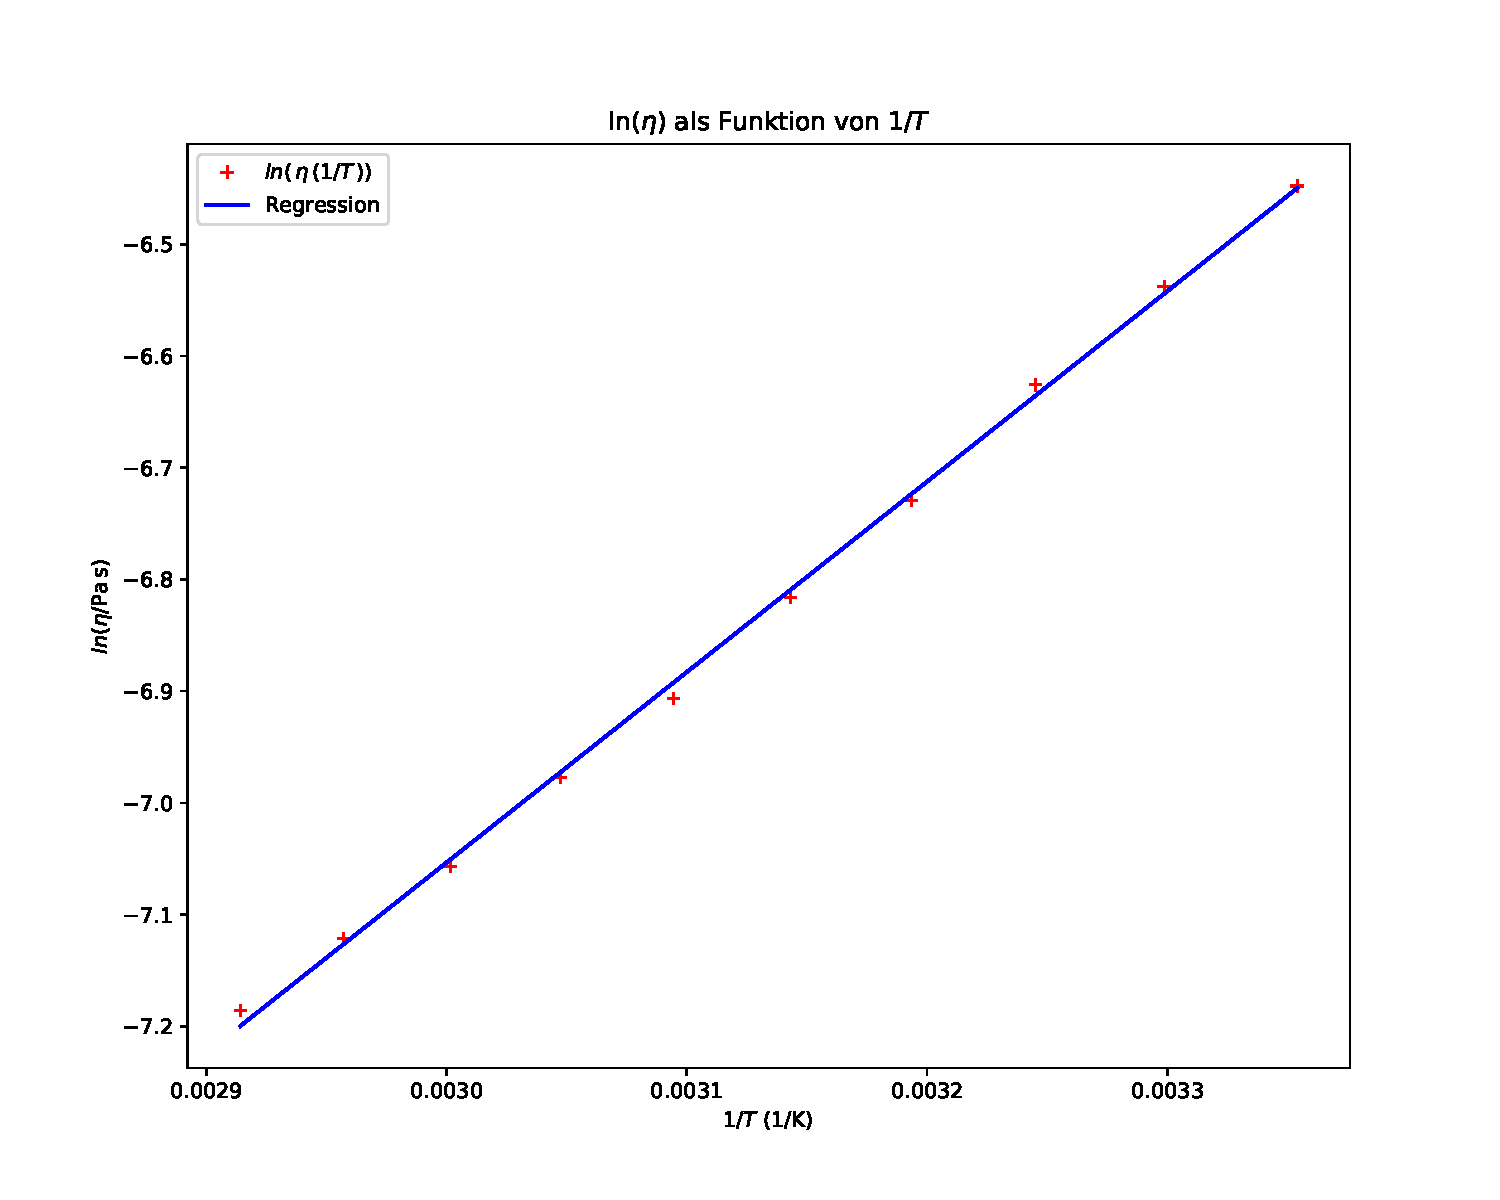
\includegraphics[scale=0.6]{etaT.pdf}
  \caption{ln($\eta$)} als Funktion von 1/T mit Regression
  \label{plot:1}
\end{figure}
Es ergeben sich folgende Koeffizienten:
\begin{equation*}
  \begin{split}
    ln(A) = \num{-12.17(7)} \\
    B = \SI{1705(21)}{\kelvin}
  \end{split}
\end{equation*}
Nach \eqref{eqn:6} ergeben sich damit Reynoldszahlen zwischen \num{33(3)} bei \SI{25}{\celsius}
und \num{149(13)} bei \SI{70}{\celsius}. Die kritische Reynoldszahl für Wasser, also die Reynoldszahl die den Übergangspunkt von
laminarer zu turbolenter Strömung charakterisiert beträgt 2000 \cite[4]{Reynold}. Die erhaltenen Werte liegen alle weit unter diesem Wert,
sodass davon ausgegengen werden kann, dass es sich immer um eine laminare Strömung gehandelt hat.
\section{Diskussion}
Beim Vergleich der gemessenen Viskositäten (siehe Tabelle \ref{tab:4}) mit Literaturwerten (\cite[1]{LitEta})
zeigen sich Abweichungen von ca. \SI{55}{\percent}, die nicht im Bereich der Messungenauigkeit liegen.
Mögliche systematische Fehlerquellen sind Luftblasen, die sich trotz des Versuches sie zu entfernen in der Apperatur gesammelt
haben können. Unterstützt wird diese These von der Tatsache, das sich eine sehr gute lineare Regression
für die Viskosität finden lässt, deren Fehler sehr gering ist. Auch die Temperaturregelung zeigte sich
als im besten Falle nur grob einzustellen, sodass die angegebenen Temperaturen nicht mit Sicherheit zu
verifizieren sind. Desweiteren betrachten die verwendeten Formeln die, wenn auch geringe, Reibung der Kugel
an den Seiten der Röhre nicht.
Turbulente Strömungen sind hingegen als Fehlerquelle auszuschließen. Die Betrachtung der Reynoldzahl zeigt eindeutig, dass das
Strömungsverhalten in der Röhre laminar war.

Zusammenfassend zeigen die gemessenen Werte untereinander schlüssige Zusammenhänge, die jedoch nicht mit der Literatur übereinstimmen.
Es sind also weitere Messreihen nötig. Eine Möglichkeit, die Messung zu verbessern, läge sicherlicher darin, den Einschluss von
Luft in der Apparatur zu verringern. Ein Befüllen im Vakuum wäre zwar technisch aufwendig, könnte die Messgüte jedoch steigern.
Weiterhin wurden bei der Hauptmessreihe pro Temperatur lediglich jeweils zwei Messwerte genommen. Hier ließen sich
durch mehrfache Messungen bessere Resultate erzielen.
\newpage
\nocite{*}
\printbibliography
